\question (南京理工大学,1997年)下列关于m阶B-树的说法中,错误的是( )
\par\twoch{根结点至多有m棵子树}{所有叶子都在同一层次}{\textcolor{red}{非叶结点至少有m/2(m为偶数)或m/2+1(m为奇数)棵子树}}{根结点中的数据是有序的}
\begin{solution}一棵m阶B树(Balanced Tree of Order
m)是一棵平衡的m路搜索树,它或者是空树,或者是满足下列性质的树:
1)若根结点不是终端结点,则根结点至少有两个子女。
2)根结点以外的所有结点(不包括失败结点)至少有m/2个子女。
3)所有的叶子结点(失败结点)都位于同一层,并且不带信息。
4)树中非叶子结点最多有m棵子树(即至多有m-1个关键字)。
5)各结点内关键字均有序排列。 因此A正确,B正确,D正确。
C选项错误,因为根结点除外,根节点至少有2个分支,非根节点至少有m/2个子女。
\end{solution}
\question (湖南大学,2003年)在一棵m阶B-树中,若在某结点中插入一个新关键字而引起该结点的分裂,则此结点中原有的关键字个数是(
)
\par\twoch{m}{m+1}{\textcolor{red}{m-1}}{m/2}
\begin{solution}树中非叶子结点最多有m棵子树(即至多有m-1个关键字)。当插入关键字使得结点关键字变为m时,就需要拆分。
\end{solution}
\question (北京交通大学,2004年)含有n个非叶子结点的m阶B-树至少包含( )个关键字
\par\twoch{(m-1)*n}{n}{n*(m/2-1)}{\textcolor{red}{(n-1)*(m/2-1)+1}}
\begin{solution}根结点至少1个关键字,其余n-1个结点至少m/2-1个关键字,因此总共至少包含(n-1)*(m/2-1)+1个关键字。
\end{solution}
\question 下列叙述中,不符合m阶B树定义要求的是( )
\par\twoch{根结点最多有m棵子树}{所有叶结点都在同一层上}{各结点内关键字均升序或降序排列}{\textcolor{red}{叶结点之间通过指针链接}}
\begin{solution}D选项是B+树的特点,而不是B树的特点。 【总结】 一棵m阶B树(Balanced Tree
of Order
m)是一棵平衡的m路搜索树,它或者是空树,或者是满足下列性质的树: ①
若根结点不是终端结点,则根结点至少有两个子女。 ②
根结点以外的所有结点(不包括失败结点)至少有⌈m/2⌉个子女。 ③
所有的叶子结点(失败结点)都位于同一层,并且不带信息。 ④
树中非叶子结点最多有m棵子树(即至多有m-1个关键字)。 ⑤
各结点内关键字均有序排列。
\end{solution}
\question 设有一棵3阶B树,如下图所示。删除关键字78得到一棵新B树,其最右叶结点所含的关键字是(
~)。

~
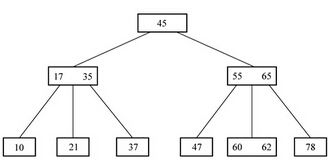
\includegraphics[width=3.26042in,height=1.60417in]{computerassets/04c0e2e1f321e7045cd7b9c52c54a6a8.jpeg}
\par\twoch{60}{60,62}{62,65}{\textcolor{red}{65}}
\begin{solution}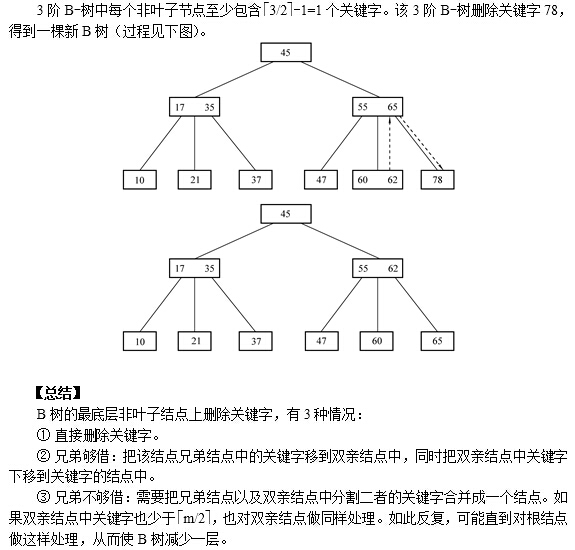
\includegraphics[width=3.33333in,height=3.18750in]{computerassets/ffad7e44985976db5df9f2ad0d25a55c.jpeg}
\end{solution}
\question 在一棵具有15个关键字的4阶B树中,含有关键词的结点个数最多是( )
\par\twoch{5}{6}{10}{\textcolor{red}{15}}
\begin{solution}本题考虑结点个数最多的极端情况,即一个结点只有一个关键字的情况,此时结点个数最多为15个。
\end{solution}
\question (哈尔冰工程大学,2005年)具有n个关键字的m阶B-树,有(
)个叶子(查找不成功)节点
\par\twoch{\textcolor{red}{n+1}}{n-1}{m*n}{[m/2]*n}
\begin{solution}考察B-树的性质,可以这样来考虑,对于非叶子结点来说,若有一个关键字,则有两个分支,两个关键字,就会产生三个分支,依次类推,每增加一个关键字,就会增加一个分支,故查找不成功的节点的个数为n+1
\end{solution}
\question (北京航空航天大学,2004年)下述命题中,不成立的是( )
\par\fourch{m阶B树中的每一个分支节点的子树的个数都小于或等于m}{\textcolor{red}{m阶B树中的每一个分支节点的子树的个数都大于或等于m/2(向上取整)}}{m阶B树中的任何一个节点的子树的高度都相等}{m阶B树中有k个子树的分支节点包含k-1个关键字}
\begin{solution}m阶B树中的每一个非根节点的子树的个数至少是m/2(向上取整),而不是每一个分支节点,根节点除外
\end{solution}
\question (华南理工大学,2006年)已知一棵5阶B树有53个关键字,并且每个节点的关键字都达到最少状态,则它的深度是(
)
\par\twoch{3}{4}{\textcolor{red}{5}}{6}
\begin{solution}根据B树定义,m阶B树除根之外所有的非终端节点至少有m/2(向上取整)个节点,即3个,而根节点最少有两个节点,在每个节点的关键字是最少状态时,5层的满树节点的关键字为1+2+3*2+3*2*3+3*2*3*3大于53,而4层满树节点关键字小于53.故深度为5
\end{solution}
\question (北京航空航天大学,2004年)下面关于B树和B+树的叙述中,不正确的是( )
\par\fourch{B树和B+树都是平衡的多分树}{B树和B+树都可用于文件的索引结构}{B树和B+树都能有效地支持随机检索}{\textcolor{red}{B树和B+树都能有效地支持顺序检索}}
\begin{solution}因为B+树所有的叶子节点中包含了全部关键字信息,以及指向含有这些关键字记录的指针,且叶子节点本身依关键字的大小自小而大顺序连接,所以支持从根节点的随机检索和从叶子节点开始的顺序检索,但是B树不具有这种结构特性,所以只支持从根节点的随机检索,而不支持直接从叶子开始的顺序检索。
\end{solution}
\question (青岛大学,2005年)在非空m阶B-树上,除根节点之外的所有其他非终端节点(
)
\par\fourch{\textcolor{red}{至少有m/2(取上整)棵子树}}{至多有m/2(取上整)棵子树}{至少有m/2(取下整)棵子树}{至多有m/2(取下整)棵子树}
\begin{solution}考察B-的性质,B-树除根节点外,每个节点至少有m/2(取上整)棵子树
\end{solution}
\question (青岛大学,2004年)m阶B-树中所有的非叶子节点(除根之外)节点中的关键字个数必须大于或者等于(
)
\par\twoch{m/2(取上整)}{\textcolor{red}{m/2(取上整)-1}}{m/2(取下整)}{m/2(取下整)-1}
\begin{solution}因为B-树除根之外的非叶子节点最少有m/2(取上整)个分支,故关键字个数必须大于或者等于m/2(取上整)-1
\end{solution}
